%/**********************************************************************/
%		第3章:LEDマトリクスパネルを用いた画像表示システムの構築
%/**********************************************************************/
\chapter{LEDマトリクスパネルを用いた画像表示システムの構築}
\label{lbl_chptr3}
本章では,LEDマトリクスパネルの基本的な仕様を理解した上で,独自の画像表示システムを構築する.256階調での画像表示システムの構築を始めとし,遠隔地から画像をアップロードして表示を行えるシステムや,ガンマ補正を適用した画像表示の品質向上を目指す.


%======================================================================
% 3.1 使用デバイスと開発環境
%======================================================================
\section{使用デバイスと開発環境}

本節では,使用したHUB75規格の 64×32 LEDマトリクスパネルのハードウェア仕様と,
小型コンピュータのRaspberry Piを中心とした開発環境についてまとめる.

\subsection{HUB75規格 64×32 LEDマトリクスの仕様}

本研究では,HUB75インタフェース規格を採用した64×32ピクセルのLEDマトリクスパネル\cite{aliexpress_hub75_led}を使用した.
HUB75は,市販のRGB LEDマトリクスが画像データを受け取るために用いる信号インターフェースである\cite{switch_science_lmcm}.
本システムでは,64列×32行の合計2,048個のRGB LEDを制御し,
各LEDは赤(R),緑(G),青(B)の3色を独立に制御できる.

HUB75インタフェースは,データ信号,クロック信号,ラッチ信号,出力イネーブル(OE)信号,
行アドレス信号などから構成され,高速な走査制御を実現する.
本システムでは,このHUB75インタフェースを用いて120 Hz相当のフレーム更新を実行し,
可視光通信の送信端末として機能させる.
使用したLEDマトリクスパネルの製品仕様を表\ref{tab:hub75_spec}に示す.

\begin{table}[H]
  \centering
  \caption{HUB75 64×32 LEDマトリクスパネルの製品仕様\protect\footnotemark}
  \label{tab:hub75_spec}
  \begin{tabular}{|p{0.48\linewidth}|p{0.48\linewidth}|}
    \hline
    \multicolumn{2}{|c|}{製品仕様} \\
    \hline
    懸念化学物質の有無 (High-concerned chemical) & なし (None) \\
    \hline
    カスタマイズ可否 (is\_customized) & はい (Yes) \\
    \hline
    ピクセル / 画素ピッチ (Pixels / Pixel pitch) & 4mm \\
    \hline
    表示機能 (Display Function) & ビデオ (VIDEO) \\
    \hline
    チューブチップの色 (Tube Chip Color) & フルカラー (Full Color) \\
    \hline
    モデル番号 (Model Number) & P4-64X32-16S or 32S \\
    \hline
    ブランド (Brand Name) & OIMG / Starlight \\
    \hline
    原産国/原産地 (Origin) & 中国(中国本土,Mainland China) \\
    \hline
    用途 (Use) & 屋内 (Indoor) \\
    \hline
  \end{tabular}
\end{table}
\footnotetext{https://ja.aliexpress.com/item/1005010223788711.html より引用.}

本実験で使用したHUB75 64×32 LEDマトリクスパネルの外観と点灯例をそれぞれ図\ref{fig:matrix_led},及び図\ref{fig:matrix_light_example}に示す.


\begin{figure}[H]
  \centering
  \includegraphics[width=0.8\linewidth]{assets/matrix_led.png}
  \caption{HUB75規格 64×32 LEDマトリクスパネルの外観\protect\footnotemark}
  \label{fig:matrix_led}
\end{figure}
\footnotetext{https://ja.aliexpress.com/item/1005010223788711.html より引用.}

\begin{figure}[H]
  \centering
  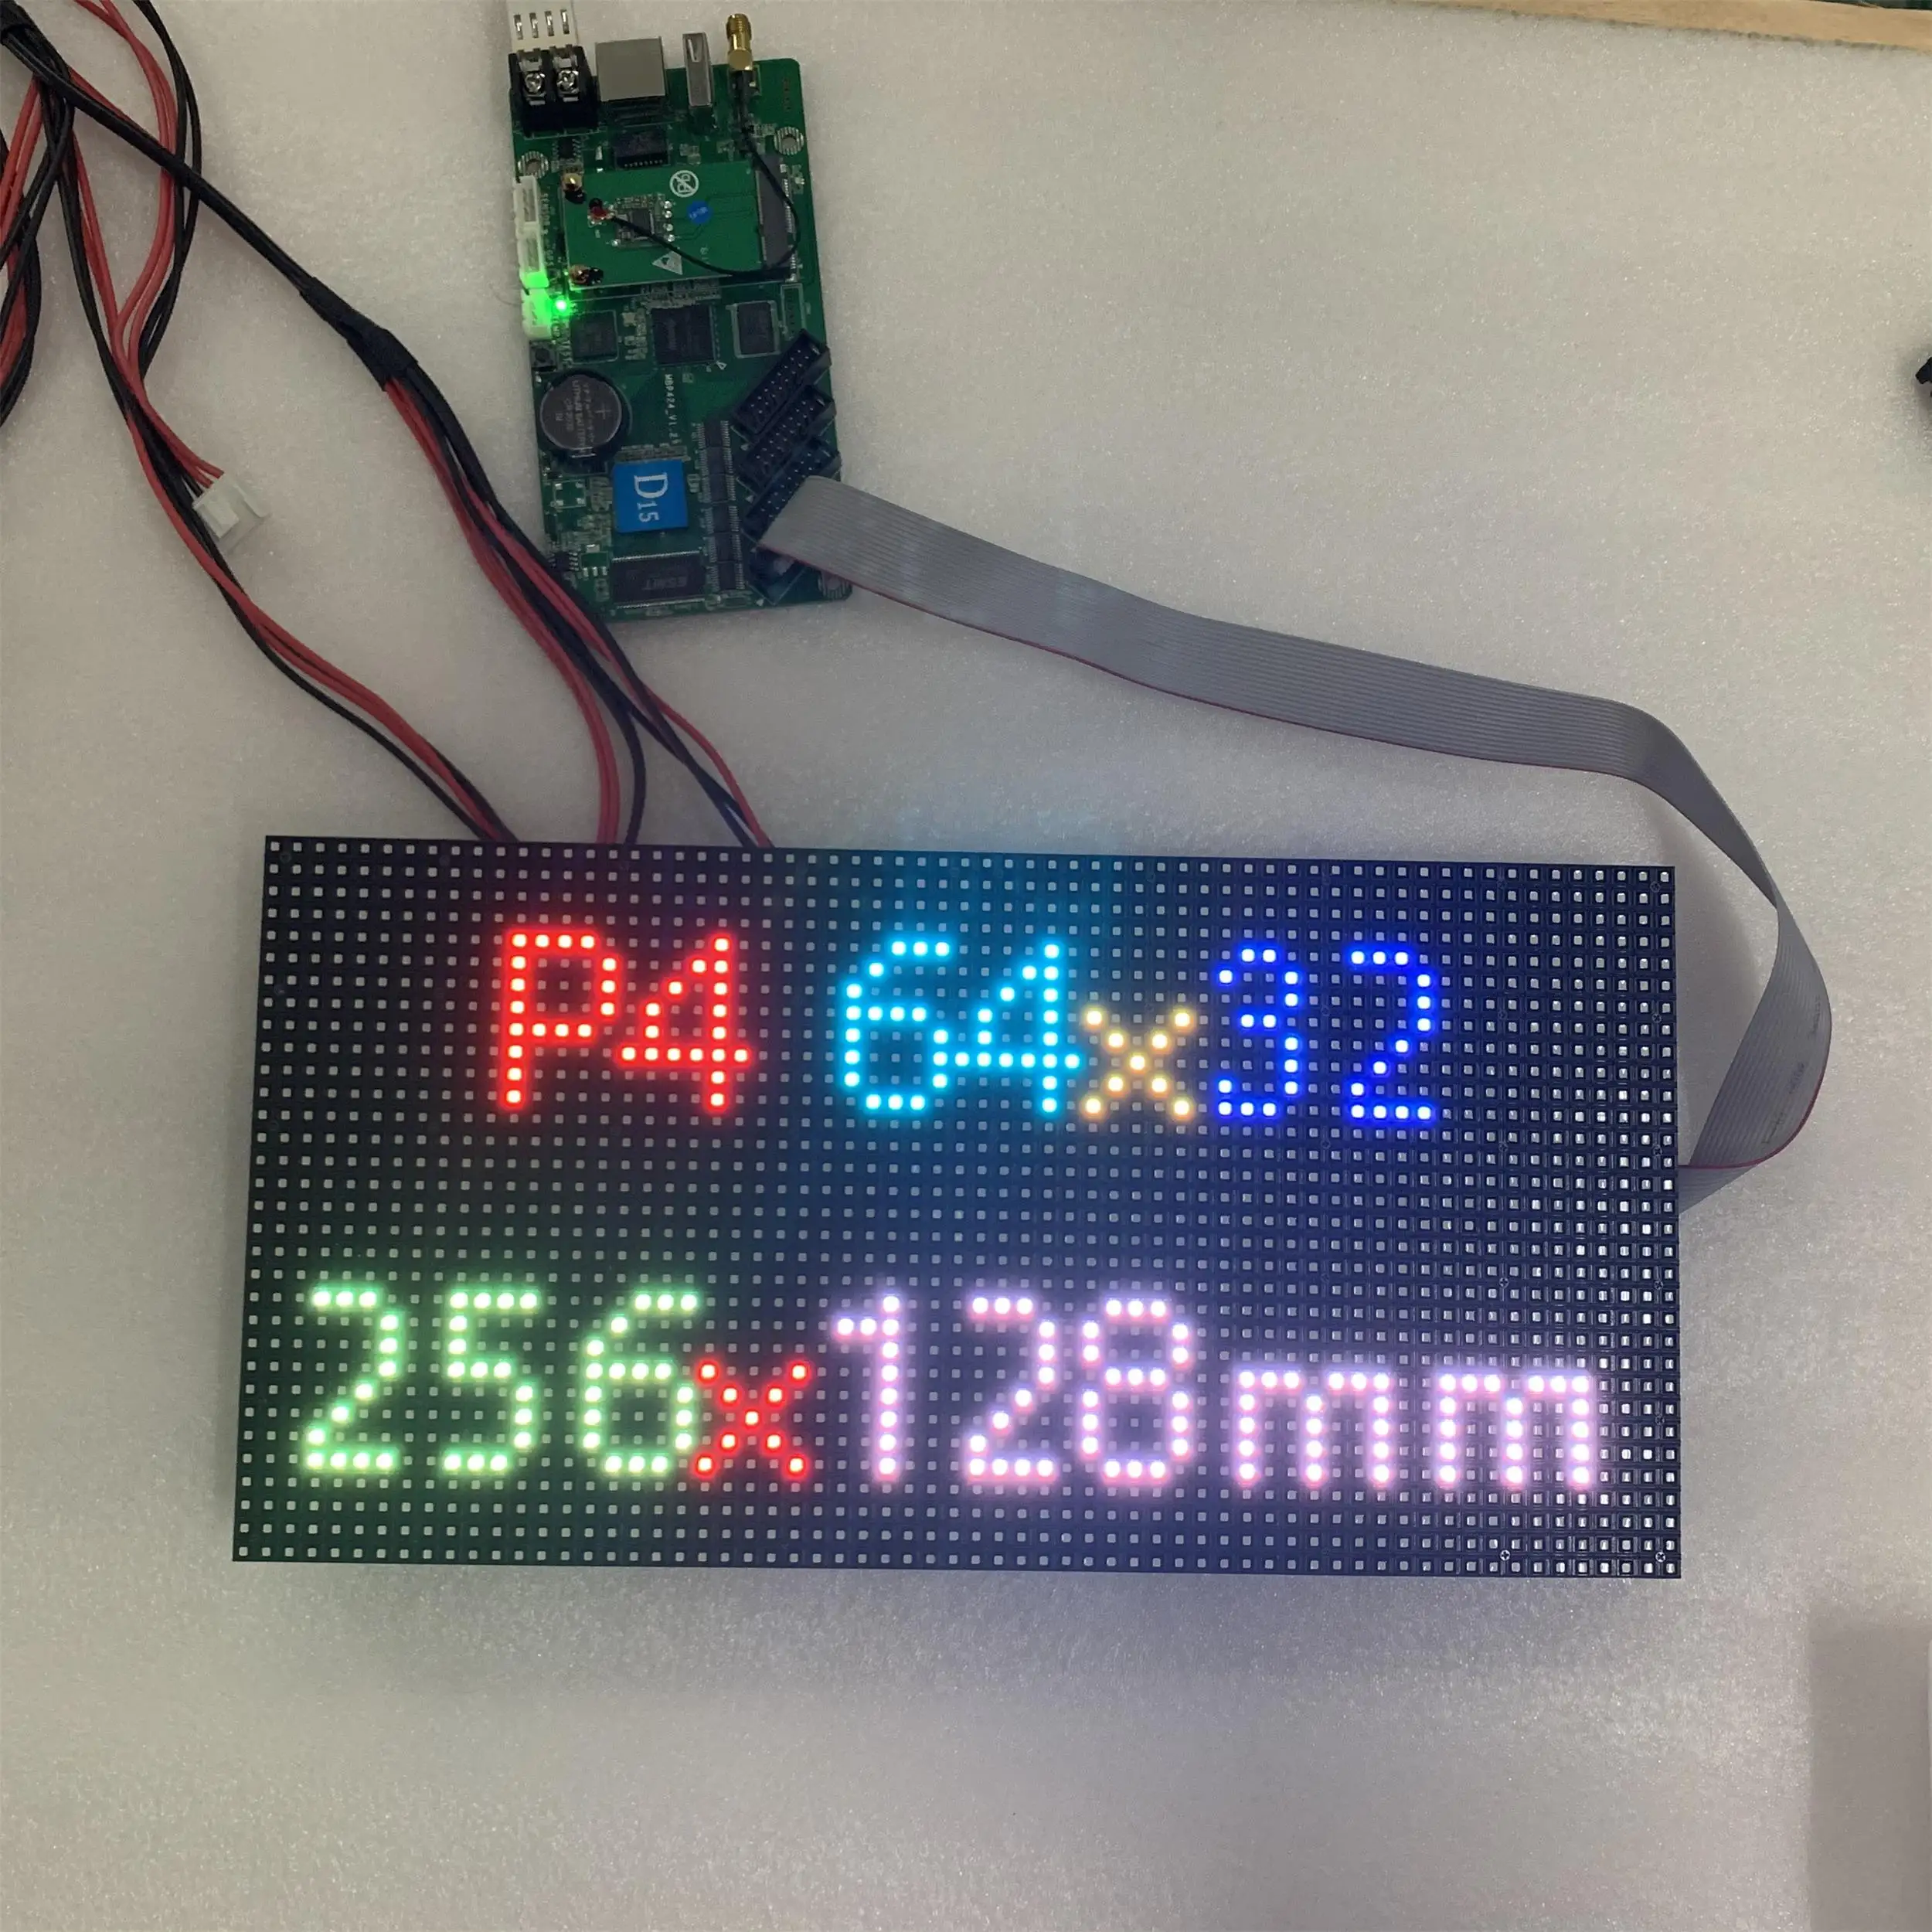
\includegraphics[width=0.8\linewidth]{assets/matrix_light_example.png}
  \caption{HUB75規格 64×32 LEDマトリクスパネルの点灯例\protect\footnotemark}
  \label{fig:matrix_light_example}
\end{figure}
\footnotetext{https://raspberry-pi.ksyic.com/?pdp.id=552 より引用.}

\subsection{Raspberry Pi 4と開発環境}

本研究では,小型コンピュータのRaspberry Pi 4 Model Bを制御用コンピュータとして使用した.
Raspberry Pi 4は,ARMアーキテクチャを採用したシングルボードコンピュータであり,
GPIO(General Purpose Input/Output)ピンを用いてHUB75インタフェースのLEDマトリクスパネルを直接制御することが可能である.
本システムでは,Raspberry Pi 4上でC言語によるLEDパネル制御プログラムを実行し,
高速な点滅制御を実現している.
また,Python環境を併用して,Webサーバの動作もRaspberry Pi 4上で実現している.

Raspberry Pi 4 Model Bの外観と主要仕様をそれぞれ図\ref{fig:raspberry_pi_外观}と表\ref{tab:raspberry_pi_spec}に示す.

\begin{figure}[H]
  \centering
  \includegraphics[width=0.8\linewidth]{assets/raspberry_pi_4.jpg}
  \caption{Raspberry Pi 4 Model Bの外観\protect\footnotemark}
  \label{fig:raspberry_pi_外观}
\end{figure}
\footnotetext{https://www.element14.com/raspberry-pi/raspberry-pi-4-model-b/dp/SC0195/item より引用.}

\begin{table}[H]
  \centering
  \caption{Raspberry Pi 4 Model Bの主要仕様\protect\footnotemark}
  \label{tab:raspberry_pi_spec}
  \begin{tabular}{|l|p{10cm}|}
    \hline
    \multicolumn{2}{|c|}{基本仕様} \\
    \hline
    販売元 & element14 \\
    \hline
    製品型番 & SC0195/0765756931199 \\
    \hline
    リビジョン & 1 \\
    \hline
    SoC & Broadcom BCM2711 \\
    \hline
    CPU & 1.5GHz クアッドコア Cortex-A72(ARMv8,64bit,L1=データ用32KB 命令用48KB/Core,L2=1MB) \\
    \hline
    GPU & デュアルコア VideoCore VI® 500MHz,OpenGL ES 3.0対応,ハードウェアOpenVG対応,H.265(HEVC)4Kp60 デコード,H.264 1080p60 デコード / 1080p30 エンコード \\
    \hline
    メモリー & 8GB LPDDR4-3200 SDRAM \\
    \hline
    電源 & USB type Cソケット 5V 3.0A / 2.54mm ピンヘッダー / PoE(要オプションPoE HAT) \\
    \hline
    消費電力(本製品単体) & アイドル:約3W,ストレス:約6.25W \\
    \hline
    サイズ & 85 × 56 × 18mm \\
    \hline
    生産国 & 英国 \\
    \hline
    \multicolumn{2}{|c|}{インターフェース} \\
    \hline
    イーサネット & 10/100/1000 Base-T RJ45 ソケット (BCM54213PE) \\
    \hline
    無線LAN(WiFi) & IEEE 802.11 b/g/n/ac 2.4/5GHz デュアルバンド (Cypress CYW43455) \\
    \hline
    Bluetooth & Bluetooth 5.0, Bluetooth Low Energy (Cypress CYW43455) \\
    \hline
    ビデオ出力 & micro HDMI ×2,コンポジット 3.5mm 4極ジャック(PAL,NTSC),DSI 2-lane(15pin 1mmピッチ) \\
    \hline
    オーディオ出力 & 3.5mm 4極ジャック,micro HDMI(ビデオ出力と共有)×2,I2Sピンヘッダー \\
    \hline
    カメラ入力 & 2-lane MIPI CSI(15pin 1mmピッチ) \\
    \hline
    USB & USB 2.0 × 2,USB 3.0 × 2 (VIA VL805 PCIe) \\
    \hline
    GPIO コネクター & 40ピン 2.54mm ピンヘッダー(GPIO×26 3.3V 16mA,UART,I2C,SPI,I2S,PWM,5V出力(使用電源に依存),3.3V出力 50mA(GPIO信号との総和)) \\
    \hline
    メモリー カード スロット & micro SDメモリーカード(SDIO) \\
    \hline
  \end{tabular}
\end{table}
\footnotetext{\texttt{https://raspberry-pi.ksyic.com/?pdp.id=552} より引用}

%======================================================================
% 3.2 256階調表示システム
%======================================================================
\section{256階調表示システム}
\label{sec:256system}
本節では,256階調表示システムの構築について説明する.256階調表示システムとは,LEDマトリクスパネル上でRGB各色をそれぞれ256段階の明るさで表現し,フルカラー画像を表示するための仕組みである.本研究では可視光通信の送信端末としてLEDマトリクスパネルを用いるため,送信する画像を視覚的に識別しやすく表示する必要があり,そのために256階調での表示を実現した.本節の構成は次のとおりである.まず,本研究で今回採用した点灯方式による256階調表現と点灯タイミングの計算方法を述べ,続いて本研究の点灯方式と一般的なPWM制御との比較を行う.その後,画像のリサイズ,及びマッピング処理から点灯制御までの処理手順を説明する.

\subsection{本研究で採用した方式による256階調表現}
\label{sec:256gradation}
RGB各色を今回採用した方式(各色を点灯する回数で輝度を表す)により256階調で表示するシステムを構築する.
HUB75では,一つのLEDでR,G,Bの3色をそれぞれ点灯させるかしないかを独立に制御が可能である.その仕様を利用して,R,G,Bそれぞれの点灯回数で256階調を表現する.
ここで用いるスロットとは,時間軸を等間隔に区切った一区間であり,その区間では「点灯する」か「点灯しない」かのどちらかしか選べない,一回の点灯判定の最小単位である.本研究の方式では,このスロットを256個用意し,そのうち何回のスロットで点灯するか(点灯回数)で輝度を表す.

例えば,図\ref{fig:gradation}の例では,暗めの青色を表現しているが,今回の暗めの青色の場合は(R,G,B)=(92,225,128)であり,この場合,256階調のうち92回Rを点灯させ,225回Gを点灯させ,128回Bを点灯させることで表現が可能である.

\begin{figure}[H]
  \centering
  \includegraphics[width=0.8\linewidth]{assets/256gradation.png}
  \caption{本研究で採用した方式による256階調表現}
  \label{fig:gradation}
\end{figure}

\subsection{一般的な点灯制御方式との比較}
\label{sec:lighting_comparison}

一般的な点灯制御方式としては,PWM制御がある.PWM制御は,一定周期のパルスのうちONになっている時間の割合(デューティ比)を変えることで見かけの明るさを変える方式である.例えばデューティ比50\%であれば1周期の半分の時間だけ点灯し,平均として中間の輝度になる.多くのマイコンやLEDドライバでは,ハードウェアまたは専用回路でPWM波形を生成し,デューティ比を輝度値に応じて設定して多階調表示を実現している.
例として図\ref{fig:pwm}に示す画像を表示する場合を考える.
\begin{figure}[H]
  \centering
  \includegraphics[width=0.8\linewidth]{assets/pwm.png}
  \caption{PWM制御による点灯制御}
  \label{fig:pwm}
\end{figure}

図\ref{fig:pwm}は図\ref{fig:gradation}と同様に$(R,G,B)=(92,225,128)$の場合を示している.
この場合,$R=92$であるためデューティ比は$92/256 \approx 36.3\,\%$で点灯させ,$G=225$は$225/256 \approx 87.8\,\%$,$B=128$は$128/256 \approx 50.0\,\%$のデューティ比でそれぞれ点灯させることで表現が可能である.

このように,PWM制御では輝度値をデューティ比に変換して点灯させることで,256階調を表現することができる.

しかしながら,本研究で採用した方式では,デューティ比ではなく,1フレームを256スロットに分割し,各スロットで点灯するか否かを整数演算で決めることで,輝度値$R$を256スロット中$R$回の点灯として表現する.点灯させるタイミングの決め方については次節で述べる.

本研究の方式はPWMと本質的には変わらず,いずれも時間あたりの点灯時間の割合で輝度を表す.相違点は,PWMがデューティ比(点灯している時間の長さ)で制御するのに対し,本研究の方式はスロットを256個用意し,そのうち何回点灯させるかという回数で制御する点である.
この違いにより,次のようなメリットがある.

第一に,輝度値が0--255の整数でそのまま点灯回数に対応するため,後述するガンマ補正後の値をそのまま使え,画像処理との接続が容易である.

第二に,\ref{lbl_chptr4}章で述べる可視光通信ではスロット単位の点灯パターンでデータを送るため,同じスロット構造を共有でき,表示と通信の両立が容易となる.

また,実装容易性の面では,PWMではハードウェアまたは専用回路でデューティ比に応じた波形を生成する必要があるのに対し,本研究の方式ではHUB75のON/OFF制御のみで,ソフトウェアで各スロットの点灯有無を整数演算で決めることが可能となる.

以上より,本研究では\ref{sec:256gradation}項の方式を採用した.

\subsection{点灯させるタイミングの計算方法}
% 本研究では1フレームを1スロットとして,256スロット(=256フレーム分)のあいだで点灯回数を制御する.したがって,1枚の画像は256フレームをかけて表現される.HUB75の仕様上,行走査とフレームという二種類の時間構造があり,その具体例を図\ref{fig:hub75_logic}に示す.

% \begin{figure}[H]
%   \centering
%   \includegraphics[width=0.8\linewidth]{assets/hub75_logic.png}
%   \caption{HUB75の行走査とフレームの時間構造}
%   \label{fig:hub75_logic}
% \end{figure}

% 図\ref{fig:hub75_logic}は,HUB75における走査の時間構造を模式的に示している.横軸は時間である.

% 本研究で用いているのは1/16走査のHUB75であり,一回の走査で2行を同時に制御する(例:1行目と17行目,2行目と18行目).32行のパネルでは16回の走査で1スロット分の点灯制御が行われる.図中の赤いパルスは,1行分の行選択期間(点灯可能な区間)を表しており,1パルスは1行に対応する.1つの赤パルスの時間幅は1フレーム時間の$1/32$であり,パルス幅とパルスがない区間の時間幅は等しい.したがって,1パルス+パルスのない1区間で1フレームの$1/16$となり,1フレームのあいだに16回の行選択が行われる.

% 輝度制御の基本単位であるスロットは,本研究では1フレームに相当する.つまり,1フレームが1スロットに該当し,各スロット(=各フレーム)ごとに点灯するかしないかを決めることで輝度を制御している.以上より,図の時間構造では「1パルス=1行」,「1フレーム=1スロット」として扱う.
本研究では1フレームを1スロットとして,256スロット(=256フレーム分)の間で点灯回数を制御する.従って,1枚の画像は256フレームをかけて表現される.その一方,単純に1フレーム内でスロットを配置するだけでなく,RGBのスロットをフレーム内で均等に配置する必要がある.その理由を説明するにあたって,RGBを均等に配置しないパターンを図\ref{fig:gradient_slot}に示す.
\begin{figure}[H]
  \centering
  \includegraphics[width=0.8\linewidth]{assets/gradient_slot.png}
  \caption{スロットが均等に配置されていないパターン}
  \label{fig:gradient_slot}
\end{figure}

この例は,シアンを表現するにあたって,RGBのスロットの均等に配置しないパターンを示している.Rが前半に集中しており,前半はRGB全てが点灯されるが,後半は赤色が配置されなくなるため,フレームの前半と後半で見える色が異なって見える.このように,フレーム内でスロットを均等に配置しないと,フレームの前半と後半で見える色が違って見えるため,画質が損なわれる可能性がある.

そこで,本研究ではスロットを均等に配置する方法を採用した.
当初は,スロットを均等に配置する方法として,整数除算でスロットの配置パターンを決める方法を検討した.

例えば,$R=128$の場合,256スロットを128で割った商は2であるため,256スロット中で2回に1回点灯することになる.しかしながら,この方法では,$R$が256の約数でない場合に,スロットを均等に配置することができない.
例えば,$R=200$の場合,256スロットを200で割った商は1であるため,256スロット中で1回に1回,つまり毎回点灯することになってしまう.

そのため,本研究で採用した方法では,各スロットごとの累積値(accumulator)に目標輝度値$R$を加算し,加算結果が256を超えたとき(オーバーフローしたとき)に点灯し,累積値を256で割った余りに更新する.これにより,$R$が256の約数でない場合でも,256スロット中$R$回の点灯を時間的に均等に分散でき,階調の線形性と画質の向上が期待できる.本研究では,スロットを均等に配置する方法として,この方法を採用した.以下,まず$R=200$の具体例を示し,続いてこの方法が成り立つ理由を述べる.

具体例として$R = 200$の場合を,図\ref{fig:my_logic}を使って説明する.

\begin{figure}[H]
  \centering
  \includegraphics[width=0.8\linewidth]{assets/my_logic.png}
  \caption{$R=200$のときの累積値の遷移}
  \label{fig:my_logic}
\end{figure}

図中の紫色の領域が累積値,水色の領域が目標輝度値$R$(この例では200)を表す.初期値は$\mathrm{acc}_0 = 0$である.

各スロットでは「累積値に200を足す」を行う.足した結果が256未満ならそのまま次の累積値とし,256以上なら点灯して256を引いた余りを次の累積値とする.図\ref{fig:my_logic}を見ると,スロット1では$0 + 200 = 200$で256未満のため点灯せず,累積値は200になる.スロット2では$200 + 200 = 400$で256以上となるため点灯し,余りは$400 - 256 = 144$なので累積値は144になる.同様に,スロット3では$144 + 200 = 344$で点灯し累積値88,スロット4では$88 + 200 = 288$で点灯し累積値32,スロット5では$32 + 200 = 232$で256未満のため点灯せず累積値232,となる.図中で累積値が「下がる」瞬間が,そのスロットで点灯したことを意味すし(256を引いたため値が小さくなる).累積値が上がる瞬間が,そのスロットで点灯しなかったことを意味する.

このように,累積値が256を超えたスロットで点灯するので,点灯列は「OFF, ON, ON, ON, OFF, ON, ON, ON, ON, OFF, ON, ON, ON, OFF, ON, $\ldots$」となる.256スロットの間にちょうど200回点灯し,かつ点灯が均等に分散するため,輝度200の階調を正しく表現できる.

次に,この方法が成り立つ理由を理論的に述べる.

$n$番目のスロット開始時点の累積値を$\mathrm{acc}_n$とし,初期値を$\mathrm{acc}_0 = 0$とする.各スロットでは,現在の累積値に$R$を加算し,加算結果が256以上であれば点灯して256を引いた余りを次の累積値とし,256未満であれば点灯せず加算結果をそのまま次の累積値とする.これを式で表すと
\begin{equation}
\mathrm{acc}_{n+1} = (\mathrm{acc}_n + R) \bmod 256
\end{equation}
となる($R$は0以上255以下の整数).ここで$\bmod 256$は256で割った余りを表す.加算結果が256以上であるとき,余りは256未満となり,そのスロットで点灯が発生したことを意味する.

256スロット中に点灯がちょうど$R$回になる理由は次の通りである.

まず.256スロットの間に累積値へ加算される量の合計は$256 \times R$である.その理由は,各スロットで$R$を1回ずつ加算する操作を256回行うためである.点灯は,累積値に$R$を加算した結果が256以上になるタイミングで発生し,そのたびに256を引いた余りを次の累積値とする.従って,256スロット中で点灯された回数を$k$回とすると,256を引く操作がちょうど$k$回行われ,差し引かれた量の合計は$256 \times k = 256k$となる.よって256スロット終了時点の累積値は$256R - 256k$と表せる.累積値は常に0以上255以下の範囲に保たれるため,$0 \le 256R - 256k < 256$が成り立つ.両辺を256で割ると$0 \le R - k < 1$となり,$k$は点灯回数なので整数である.この不等式を満たす整数$k$は$k = R$のみである.したがって,256スロット中の点灯回数はちょうど$R$回である.

点灯が時間的に均等に配置される理由は次の通りである.

累積値を$\mathrm{acc}$と書く.各スロットでは$\mathrm{acc} \leftarrow \mathrm{acc} + R$とし,$\mathrm{acc} \ge 256$のとき点灯して$\mathrm{acc} \leftarrow \mathrm{acc} - 256$とする.従って$\mathrm{acc}$は,スロットごとに$+R$され,$\mathrm{acc} \ge 256$になるたびに点灯して,$\mathrm{acc}$が0以上255以下の値に更新される,という動きを繰り返す.つまり「次の点灯」が起こるのは,$\mathrm{acc}$が再び$256$に達するときである.

点灯直後の余りを$r$($0 \le r \le 255$)とする.次に$256$に達するまでに必要な加算量は$256 - r$である.1スロットあたりの加算量は$R$なので,点灯と点灯のあいだのスロット数$n$は
\begin{equation}
n = \left\lceil \frac{256 - r}{R} \right\rceil
\end{equation}
となる.$0 \le r \le 255$より
\begin{equation}
\label{eq:slot_range}
1 \le n \le \left\lceil \frac{256}{R} \right\rceil
\end{equation}
が成り立つ.$R$が256の約数ならば$256/R$は整数であり,$n = 256/R$が常に成り立つので,点灯はちょうど$256/R$スロットごとに起こる.$R$が256の約数でない場合でも,$n$は式(\ref{eq:slot_range})の範囲に収まり,いずれも$256/R$の前後である.このように,毎スロット同じ$R$を加算し「$256$に達したら点灯して余りに更新する」という規則そのものが,点灯を時間軸上に可能なかぎり均等に並べる.以上より,本方法により256スロット中$R$回の点灯が保証され,かつ均等に配置されることが示される.実際に点灯する画像を図\ref{fig:sky},整数除算でスロット配置を決める方式で点灯させ,ランダムなタイミングで撮影を行った画像を図\ref{fig:uneven_1},及び\ref{fig:uneven_2},本実験で採用した累積値でスロットを配置させる方式で点灯させ,ランダムなタイミングで撮影を行った画像を図\ref{fig:even_1},及び\ref{fig:even_2}に示す.

\begin{figure}[H]
  \centering
  \includegraphics[width=0.8\linewidth]{assets/sky.jpg}
  \caption{LEDマトリクスパネルに表示した元画像}
  \label{fig:sky}
\end{figure}

\begin{figure}[H]
  \centering
  \includegraphics[width=0.8\linewidth]{assets/uneven_1.jpg}
  \caption{整数除算でスロット配置を決める方式の場合1}
  \label{fig:uneven_1}
\end{figure}

\begin{figure}[H]
  \centering
  \includegraphics[width=0.8\linewidth]{assets/uneven_2.jpg}
  \caption{整数除算でスロット配置を決める方式2}
  \label{fig:uneven_2}
\end{figure}

\begin{figure}[H]
  \centering
  \includegraphics[width=0.8\linewidth]{assets/even_1.jpg}
  \caption{累積値でスロットを配置した場合1}
  \label{fig:even_1}
\end{figure}

\begin{figure}[H]
  \centering
  \includegraphics[width=0.8\linewidth]{assets/even_2.jpg}
  \caption{累積値でスロットを配置した場合2}
  \label{fig:even_2}
\end{figure}

これらの前提として,図\ref{fig:uneven_1},\ref{fig:uneven_2},\ref{fig:even_1},及び\ref{fig:even_2}は,撮影タイミングによる見え方の差が生じやすいよう,パネルを1,000 Hzという比較的低い駆動周波数で駆動した条件下で撮影したものである.

図\ref{fig:uneven_1},及び\ref{fig:uneven_2}では,整数除算でスロットの配置を決める方式で点灯させ,ランダムなタイミングで撮影を行った画像であるが,タイミングによって映るものが全く違うことが確認できる.一方で,図\ref{fig:even_1},及び\ref{fig:even_2}は,累積値でスロットを配置させる方式で点灯させ,ランダムなタイミングで撮影を行った画像であるが,この方式では,タイミングによって映るものがあまり変化しないことが確認できる.その理由は,累積値でスロットを配置させる方式では,スロットの配置が均一になるため,どのタイミングで撮影しても映るものに差がないためである.

\subsection{32×64画像へのリサイズとマッピング処理}
\label{sec:resize}
一般にSNS等で扱う画像は,1,920×1,080や1,280×720などの大きさであるが,今回使用するLEDマトリクスパネルのサイズは32×64であるため,一般的な画像をLEDマトリクスパネルに画像を表示するにあたってリサイズが必要である.
今回は32×64の画像へリサイズするにあたり,各出力ピクセルが元画像上で占める領域を求め,その領域に含まれる画素のRGB値を単純平均する方法(ボックス平均)を採用した.具体的には,出力画像の座標$(x,y)$($0 \leq x < 64$,$0 \leq y < 32$)に対して,元画像の幅を$W$,高さを$H$とすると,対応する入力領域を
\begin{equation}
x_0 = \left\lfloor \frac{xW}{64} \right\rfloor, \quad x_1 = \left\lfloor \frac{(x+1)W}{64} \right\rfloor, \quad y_0 = \left\lfloor \frac{yH}{32} \right\rfloor, \quad y_1 = \left\lfloor \frac{(y+1)H}{32} \right\rfloor
\end{equation}
で定義し,この矩形領域$[x_0, x_1) \times [y_0, y_1)$に含まれる全画素のRGB値を加算して画素数で除算することで,出力画素の値を得る.RGBの各成分は独立に平均し,
\begin{eqnarray}
R'(x,y) &=& \frac{1}{N} \sum_{(i,j) \in \Omega(x,y)} R(i,j) \\
G'(x,y) &=& \frac{1}{N} \sum_{(i,j) \in \Omega(x,y)} G(i,j) \\
B'(x,y) &=& \frac{1}{N} \sum_{(i,j) \in \Omega(x,y)} B(i,j)
\end{eqnarray}
とした.ここで$\Omega(x,y)$は上記入力領域に含まれる画素集合,$N$はその画素数である.リサイズ後のRGB値は,C言語上で定義したRGB構造体配列に格納し,LEDマトリクスパネル表示処理に入力する.

実際に図\ref{fig:origin_cat}の画像をリサイズした結果を図\ref{fig:resized_cat}に示す.

\begin{figure}[H]
  \centering
  \includegraphics[width=0.8\linewidth]{assets/origin_cat.jpg}
  \caption{元画像}
  \label{fig:origin_cat}
\end{figure}

\begin{figure}[H]
  \centering
  \includegraphics[width=0.8\linewidth]{assets/output_0.45.png}
  \caption{リサイズ後の画像}
  \label{fig:resized_cat}
\end{figure}

%======================================================================
% 3.3 表示品質評価
%======================================================================
\section{ガンマ補正による画質改善}
\label{sec:gamma}
本節では,\ref{sec:256system}節までの処理で,LEDマトリクスパネルに画像を表示した際に色が淡くなり形状が明確でない問題(図\ref{fig:resized_cat})について原因を調査し,ガンマ補正を行って画質を改善する方法について説明する.

\subsection{ガンマ補正}
ガンマとは,コンピュータの画像処理においては中間調(グレー)の明るさを示す用語であり,各機器には固有の発色特性(ガンマ特性)があり,入力された色情報をそのまま素直に出力できない\cite{eizo_gamma}.色情報の入力を$x$,出力を$y$,ガンマ値を$\gamma$とすると,
\begin{equation}
\label{eq:gamma_basic}
y = x^\gamma
\end{equation}
で表される.機器側のガンマ特性に合わせて色情報を調整して帳尻を合わせる仕組みをガンマ補正と呼ぶ\cite{eizo_gamma}.

図\ref{fig:gamma_explain}では,ガンマ補正の原理を示している.通常の画像ファイルにはガンマ0.45の補正がかかっており,この補正によって見た目よりも淡いデータとして保存されている.これを式で説明する.意図する明度(線形な光の強さ)を$L$($0 \le L \le 1$),画像ファイルに保存された値を$s$とすると,ガンマ0.45の符号化は$s = L^{1/2.2} = L^{0.45}$である.この$s$をディスプレイに入力すると,ディスプレイは式(\ref{eq:gamma_basic})の関係で$\gamma = 2.2$の補正をかけて出力する.つまり出力$y$は
\begin{equation}
  y = s^{2.2} = (L^{0.45})^{2.2} = L^{0.45 \times 2.2} = L^{0.99} \approx L
\end{equation}
となる.従って,画像ファイルでのガンマ0.45とディスプレイでのガンマ2.2が打ち消し合い($0.45 \times 2.2 \approx 1$),最終的に発光強度$y$が元の明度$L$にほぼ比例する.このため見た目の明度が線形に再現される.

\begin{figure}[H]
  \centering
  \includegraphics[width=0.8\linewidth]{assets/gamma_explain.jpg}
  \caption{ガンマ補正の原理\protect\footnotemark}
  \label{fig:gamma_explain}
\end{figure}
\footnotetext{\texttt{https://www.eizo.co.jp/eizolibrary/other/itmedia02\_07/} より引用}

このように,通常のディスプレイではガンマ2.2の補正が行われているため,画像ファイルは内部的にガンマ0.45の補正が行われている.しかしながら,LEDマトリクスパネルではこの補正が行われないため,ガンマ0.45のまま表示することになり,元の画像よりも淡く表示される問題が発生していた.この問題を可視化したものが図\ref{fig:matrix_gamma}である.

\begin{figure}[H]
  \centering
  \includegraphics[width=0.8\linewidth]{assets/matrix_gamma.png}
  \caption{LEDマトリクスパネルでのガンマ特性}
  \label{fig:matrix_gamma}
\end{figure}

図\ref{fig:matrix_gamma}をから分かる通り,LEDマトリクスパネルにはガンマ特性がないため線形となり,入力された値をそのまま出力する.そのため,ガンマ0.45に変換されている画像をそのまま出力することで淡いまま出力してしまう.

そこで本研究では,LEDマトリクスパネル上で元画像と近い見た目を得るために,画像データをパネルへ出力する前段で逆ガンマ補正(ガンマデコード)を行った.具体的には,リサイズ後の各画素のRGB値(0--255)を0--1の範囲に正規化し,各成分$s$に対して
\begin{equation}
L = s^{2.2}
\end{equation}
を適用したうえで,再び0--255にスケーリングして整数化し,LED表示用のRGB構造体配列に格納した.実装上は,画素値$R$,$G$,$B$をそれぞれ
\begin{equation}
s_R = \frac{R}{255}, \quad s_G = \frac{G}{255}, \quad s_B = \frac{B}{255}
\end{equation}
とし,
\begin{eqnarray}
R' &=& \mathrm{round}(255 \cdot s_R^{2.2}) \\
G' &=& \mathrm{round}(255 \cdot s_G^{2.2}) \\
B' &=& \mathrm{round}(255 \cdot s_B^{2.2})
\end{eqnarray}
として求めている.これにより,通常はディスプレイ側で行われているガンマ2.2の補正をソフトウェア側で補い,LEDマトリクスパネル上でも元画像に近い明度分布を再現できるようにした.実際にこの方法でガンマ補正を行った結果は以下の図\ref{fig:gamma_2.2}の通りである.

\begin{figure}[H]
  \centering
  \includegraphics[width=0.8\linewidth]{assets/output_2.2.png}
  \caption{ガンマ2.2補正画像}
  \label{fig:gamma_2.2}
\end{figure}

また,ガンマ補正をしてない状態でパネルに表示した結果を図\ref{fig:non_gamma},ガンマ補正したものをパネルに表示した結果は図\ref{fig:panel_gamma_2.2}の通りである.

\begin{figure}[H]
  \centering
  \includegraphics[width=0.8\linewidth]{assets/non_gamma.jpg}
  \caption{ガンマ補正なしの画像(パネル表示)}
  \label{fig:non_gamma}
\end{figure}

\begin{figure}[H]
  \centering
  \includegraphics[width=0.8\linewidth]{assets/display_2.2.jpg}
  \caption{ガンマ2.2補正画像(パネル表示)}
  \label{fig:panel_gamma_2.2}
\end{figure}

実際にパネルに表示した結果を見ると,ガンマ2.2補正を行ったことで,補正を行っていない画像よりもより鮮明に綺麗に表示されていることが確認できた.

%======================================================================
% 3.4 画像アップロードシステムとネットワーク構成
%======================================================================
\section{画像アップロードシステムとネットワーク構成}

本研究では,LEDマトリクスパネルを可視光通信の送信端末として用いることを目指している.送信する画像や表示内容を変更するたびにパネル設置場所へ赴くのは非効率であり,様々な画像で表示を切り替えながら視覚的に確認する実験には不向きである上,実用化後の利便性も損なわれる.そこで,遠隔地から画像をアップロードしてパネルに表示できるようにすることで,研究者や利用者がパネルに物理的に近づかずに表示内容を更新でき,可視光通信の実験や応用を柔軟に進められるようにする.

本節では,遠隔地から画像をアップロードしてLEDマトリクスパネルに表示するための
Webアプリケーションとネットワーク構成について説明する.あわせて,画像処理とLEDマトリクスパネル制御を担う実行ファイルについても説明する.

\subsection{画像処理やLEDマトリクスパネル制御用の実行ファイル}
\label{sec:execfile}

本システムでは,C言語で作成した実行ファイルが画像処理とLEDマトリクスパネルの点灯制御を担っている.
Webアプリケーションの一つであるDjango\cite{django}から実行ファイルに画像が渡され,実行ファイル内でリサイズしたのち,LEDマトリクスパネルへの点灯制御を行うまでの流れを図\ref{fig:flow_exec_file}に示す.

\begin{figure}[H]
  \centering
  \includegraphics[width=0.8\linewidth]{assets/flow_exec_file.png}
  \caption{Djangoから実行ファイルへの画像の流れと実行ファイル内での処理(リサイズ・点灯制御)}
  \label{fig:flow_exec_file}
\end{figure}

実行ファイルが行う処理のうち,画像処理としては\ref{sec:resize}節で述べるリサイズがある.PNGやJPGなどでアップロードされた画像はもともと任意の縦横ピクセル数を持つが,今回使用したLEDマトリクスパネルは64列×32行であるため,実行ファイル内で画像を64×32ピクセルにリサイズする処理を行っている.
また,点灯制御としては\ref{sec:256gradation}節で述べる256階調表現がある.実行ファイルはRaspberry PiのGPIO(General Purpose Input/Output)を制御し,HUB75インタフェースを通じてLEDマトリクスパネルに点灯パターンを送ることで,RGB各色の点灯回数により256階調で表示する.

\subsection{Webアプリケーションの構成}

画像のアップロードと表示制御のためのWebアプリケーションとして,
Djangoフレームワークを用いたWebサーバを構築した.
Django\cite{django}はPythonで記述されたWebフレームワークであり,
画像アップロード,ファイル管理,APIエンドポイントの実装が容易となる.
本システムではDjangoを用いて画像アップロード用のWebインタフェースを提供し,
アップロードされた画像をLEDマトリクスパネルに表示する.

本システムが提供するWebインタフェースとその処理の流れを図\ref{fig:web_interface}に示す.
\begin{figure}[H]
  \centering
  \includegraphics[width=0.8\linewidth]{assets/web_interface.png}
  \caption{Django WebアプリケーションのWebインタフェース}
  \label{fig:web_interface}
\end{figure}

DjangoはRaspberry Pi上でポート8000番のサーバとして動作し,常に外部からのリクエストを受け付けている.
図\ref{fig:web_interface}中のgetはGETリクエストを指し,Djangoはこれを受信すると外部データベースに問い合わせ,現在パネルに表示中の画像を取得して返却する.これはWebサイト上での表示に必要な処理となる.
postは,新たな画像をアップロードする際に用いるPOSTリクエストを指す.POSTリクエストでアップロードされた画像はサーバーレスデータベースのNeon\cite{neon}に保存したのち,Raspberry Pi 4上で実行ファイルにより処理される.実行ファイルによる処理内容は\ref{sec:execfile}節の通りである.

\subsection{Cloudflare Tunnelによる外部アクセス}

本システムでは,クラウドシステムの1つであるCloudflare Tunnel\cite{cloudflare_tunnel}を用いてRaspberry Pi 4上で動作する
Django Webアプリケーションに外部からアクセスできるようにした(図\ref{fig:cloudflare_tunnel}).
\begin{figure}[H]
  \centering
  \includegraphics[width=0.8\linewidth]{assets/cloudflare_tunnel.png}
  \caption{Cloudflare Tunnelの概要図}
  \label{fig:cloudflare_tunnel}
\end{figure}
Cloudflare Tunnelは,Cloudflareが提供するトンネリングサービスであり,
パブリックIPアドレスやポート開放なしに,ローカルネットワーク内のサービスを
インターネット経由でアクセス可能にする.
これにより,Raspberry Pi 4が設置されているローカルネットワークの設定を変更することなく,
外部のPCやスマートフォンからブラウザ経由で画像をアップロードし,
LEDマトリクスパネルに表示することが可能となった.

\subsection{Webサイトの構築}

今回は,独自でWebサイトを構築した.なお,Webサイトをインターネット上に公開するにはVercel\cite{vercel}というサービスを使用した.実際に構築したWebサイトの画面を図\ref{fig:web_site_origin}に示す.

\begin{figure}[H]
  \centering
  \includegraphics[width=0.8\linewidth]{assets/web_site_origin.png}
  \caption{Webサイトの画面}
  \label{fig:web_site_origin}
\end{figure}
このサイトでは,画像をアップロードして,パネルに表示することができる.サイト内で画像ファイルをアップロードするとその画像はBase64\footnote{Base64は,画像データなどを英数字の並びに変換する方式である.画像を文字列として送受信する際に用いられる.}形式にエンコードされ,Raspberry Piで構築しているDjango Webアプリケーションに送信される.Django Webアプリケーションでは,常にREST API\footnote{REST APIは,Web上でデータを取得したり送信したりするときのやり取りの決まりに沿った方式である.ブラウザとWebサーバの間でデータのやり取りを行う際に広く用いられる.}でリクエストを受け付け,WebサイトからBase64形式の画像を受け取ってデコードしたのち,実行ファイル(\ref{sec:execfile}節で述べる,C言語で作成したプログラム)を呼び出すようにした.実行ファイルによる処理内容は\ref{sec:execfile}節の通りである.
これにより,Webサイトから画像をアップロードして,パネルに表示することができるようになった.


\subsection{Webサイトからの画像アップロード〜パネル表示までの処理フロー}

本システムでは,Webサイトから画像をアップロードして,パネルに表示するシステムを構築した.
これにより,遠隔地から画像をアップロードしてパネルに表示することが可能となった.
本システムの全体構成を図\ref{fig:cloudflare_system}に示す.
\begin{figure}[H]
  \centering
  \includegraphics[width=0.8\linewidth]{assets/cloudflare_system.png}
  \caption{システム全体の構成}
  \label{fig:cloudflare_system}
\end{figure}
ユーザは,PCやスマートフォンのWebブラウザからCloudflare Tunnel経由で
Django Webアプリケーションにアクセスし,画像をアップロードする.
アップロードされた画像は,Raspberry Pi 4上にある実行ファイルによって実行され,\ref{sec:execfile}節で説明した通りの処理を行う.
この一連の処理フローにより,遠隔地からでもLEDマトリクスパネルの表示内容を制御することが可能となっている.
以下,Webサイトでの操作からパネル表示までの流れを,図\ref{fig:web_site_before},\ref{fig:web_site_after},及び\ref{fig:display_image}を用いて詳しく説明する.

\begin{figure}[H]
  \centering
  \includegraphics[width=0.8\linewidth]{assets/web_site_origin.png}
  \caption{アップロード前のWebサイトの画面}
  \label{fig:web_site_before}
\end{figure}

\begin{figure}[H]
  \centering
  \includegraphics[width=0.8\linewidth]{assets/web_site.png}
  \caption{アップロード後のWebサイトの画面}
  \label{fig:web_site_after}
\end{figure}

\begin{figure}[H]
  \centering
  \includegraphics[width=0.8\linewidth]{assets/display_2.2.jpg}
  \caption{LEDマトリクスパネルに表示された画像}
  \label{fig:display_image}
\end{figure}

図\ref{fig:web_site_before}は画像をアップロードする前のWebサイトの画面である.ユーザーはこの画面から画像ファイルを選択し,アップロード操作を行う.アップロードが完了すると,Webサイトの画面は図\ref{fig:web_site_after}のように更新される.この時点で,アップロードされた画像はDjango Webアプリケーションを経てRaspberry Pi上の実行ファイルに渡されている.
図\ref{fig:display_image}は,上記の処理を経た画像がLEDマトリクスパネルに実際に表示された結果である.Webサイトからアップロードした画像が,リサイズとガンマ補正を伴う点灯制御を経て,パネル上に表示されている様子が確認できる.以上が,Webサイトからの画像アップロードからパネル表示に至る一連の流れである.